\documentclass{article}

\usepackage[utf8]{inputenc}
\usepackage{enumitem}
\usepackage{todonotes}
\usepackage[ngerman]{babel}
\usepackage{amsmath}
\usepackage{float}

% Roman numerals: \rom{123}
\makeatletter
\newcommand*{\rom}[1]{\expandafter\@slowromancap\romannumeral #1@}
\makeatother

\title{Blatt 9}
\author{Luca Krüger, Jonas Otto, Jonas Merkle (Gruppe R)}
\date{\today}

\begin{document}
\maketitle
\section{Gewichtsinitialisierung}
\begin{enumerate}
  \item   \begin{enumerate}[label=\alph*)]
          \item $u_i^{(1)}$ ist normalverteilt mit $\mathcal{N}(0, \sqrt{\frac{m}{2}})$.
          \item Durch die Verwendung von $\tanh$ als Transferfunktion ändert sich die Ausgabe der
                Neuronen bei Änderung des bereits relativ großen $u_i$ kaum,
                die Ableitung $f'(u_i) \rightarrow 0$.
                Die Errorfunktion ist wie in a) ebenfalls über die Summe über die Gewichte $w_1,\dots,w_n$ definiert.
                Dies führt dann zu großen Lernschritten, da gilt $E(w)\propto \mathcal{N}(0,\sqrt{\frac{m}{2}})$\\
          \item $u_i^{(1)}$ ist normalverteilt mit $\mathcal{N}(0, \frac{1}{\sqrt{2}})$.
          \item Alle Potentiale $u_i$ liegen in einem Bereich, in dem $f'(u)$ deutlich von 0
                verschieden ist. Die Gewichte werden dadurch nicht mit Extremwerten initialisiert, die statistisch zwar selten, aber eben doch auftreten können.
        \end{enumerate}
  \item Verteilung A passt zu Strategie \rom{1}, da in Verteilung A die Gradienten alle $\approx 0$
        sind und die axonalen Potentiale 1 oder $-1$,  was auf ein betragsmäßig großes Argument
        der $\tanh$ Aktivierungsfunktion hindeutet.
        Verteilung B entspricht der skalierten Normalverteilung. Die Gradienten sind von 0 verschieden
        und die axonalen Potentiale nahezu gleichverteilt.
\end{enumerate}

\section{Regularisierung}
\begin{enumerate}
  \item Einfluss auf Lernregeln
        \begin{enumerate}[label=\alph*)]
          \item \begin{align*}
                  \frac{dE}{dw}   & =\nabla E_0\left(w(t)\right)+\lambda w(t)                             \\
                  \implies w(t+1) & = w(t) - \eta \nabla E_0\left(w(t)\right)-\eta \lambda w(t)           \\
                                  & =(1-\eta \cdot \lambda) w(t) - \eta \cdot \nabla E_0\left(w(t)\right)
                \end{align*}
          \item \begin{enumerate}[label=\roman*.]
                  \item $w(n) = 2 \cdot 0.6^n$, $w(10)=0.012$
                  \item Das Gewicht nimmt exponentiell ab.
                  \item Für $\eta\cdot\lambda < 1$ gilt:
                        \begin{equation*}
                          \lim_{t\rightarrow \infty} w(t) = \lim_{t\rightarrow \infty} w(0)\cdot (\eta \cdot \lambda)^t = 0
                        \end{equation*}
                  \item
                        $\nabla E_0(w(t))\neq0$ gilt auch für $t\to \infty$, somit gilt keineswegs $\lim_{t\to \infty} w(t)=0$
%                        In diesem Fall strebt $w(t)$ ein Minimum der Fehlerfunktion $E_0$ per Gradientenabstieg an. Die Update Regel enthält nun den Term $-\eta\cdot\nabla E_0\left(w(t)\right) \neq 0$.
                \end{enumerate}
                \item Durch den Regularisierungsterm werden die Gewichte in jedem Schritt reduziert, auch wenn $\nabla E \approx 0$ gilt. Dadurch bewegen sich die suboptimal initialisierten Gewichte schnell in sinnvollere Bereiche.
        \end{enumerate}
        \item Der Term für das Update des Bias enthält im Gegensatz zum Term für das Gewicht den Faktor $x_\mu$ nicht. Verrauschter Input wirkt sich also bereits mit der bekannten Lernregel nicht direkt auf den Bias aus.
        Starkes Rauschen wird sogar durch $f(wx + b)\cdot f'(wx + b)$ geglättet.
        
        \item Mit größerem $\lambda$ nähert sich die Errorfunktion $|w|^2$ an:
                \begin{figure}[H]
                  % body of the figure
                  \centering
                  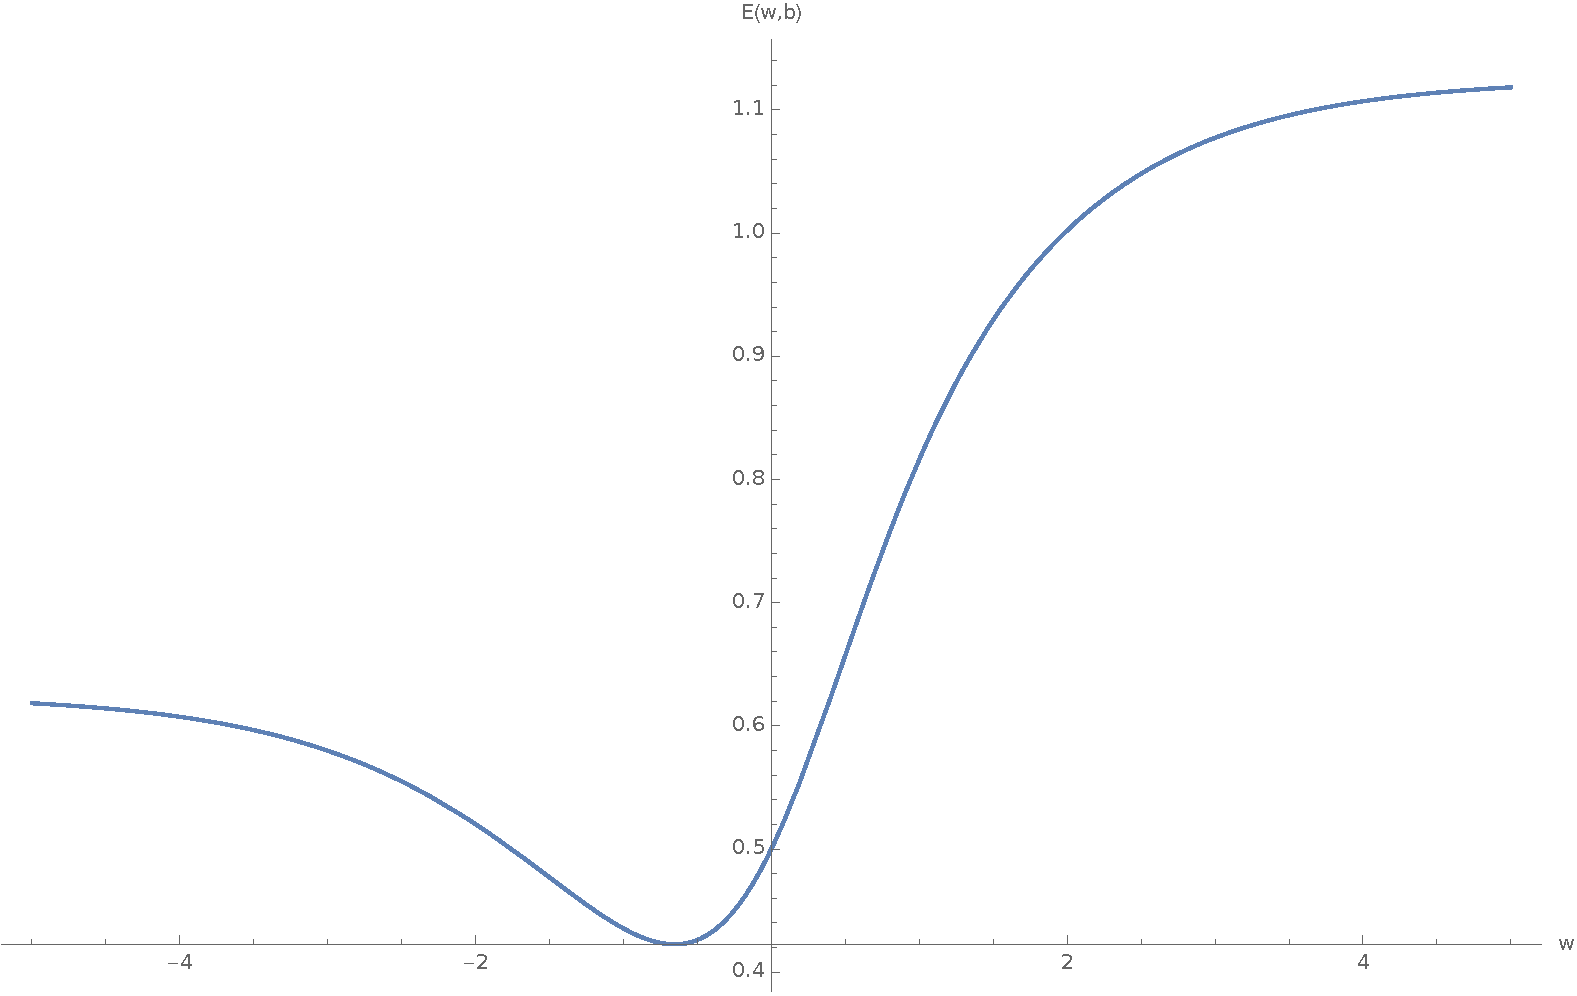
\includegraphics[width=\textwidth]{Errorfunction1.pdf}
                  \caption{Errorfunktion mit $\lambda=0$}
                \end{figure}
                \begin{figure}[H]
                  % body of the figure
                  \centering
                  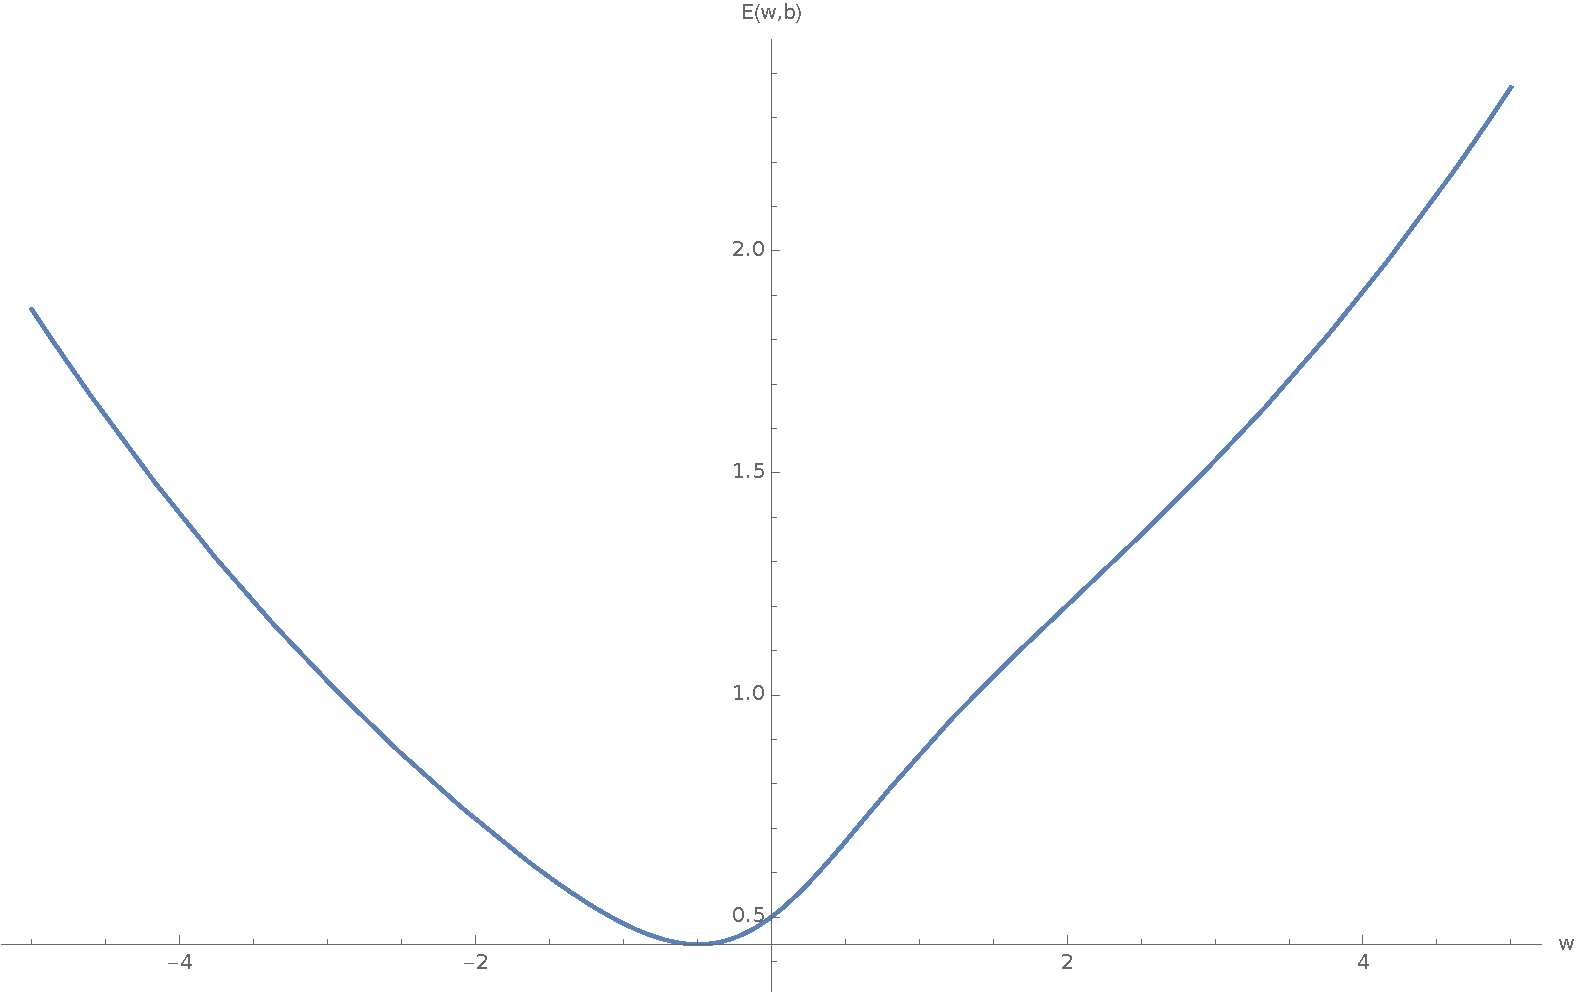
\includegraphics[width=\textwidth]{Errorfunction2.pdf}
                  \caption{Errorfunktion mit $\lambda=0.2$}
                \end{figure}
        \item (Siehe Jupyter Notebook)
\end{enumerate}


\end{document}
